\documentclass[a4paper,landscape]{article}

\usepackage[utf8]{inputenc}
\usepackage[lighttt]{lmodern}
\usepackage{amsmath}
\usepackage{amssymb}
\usepackage{amsthm}
\usepackage{listings}
\usepackage{parskip}
\usepackage{multicol}
\usepackage[margin=0.5cm,landscape]{geometry} % We dont want fat margins
\usepackage[fontsize=8pt]{scrextend} % Use a small font
\usepackage{enumitem}
\usepackage{tikz}

\usepackage{titlesec}
\titlespacing*{\section}{0pt}{0pt}{0pt}
\titlespacing*{\subsection}{0pt}{0pt}{0pt}

% Enumerate spacing
\setlist{itemsep=1pt, parsep=1pt, topsep=0pt}

% Don't print section numbers
\setcounter{secnumdepth}{0}

% Spacing between lines
\linespread{0.8}

% Remove spacing around align and between operators i math mode
% see http://tex.stackexchange.com/questions/41913/how-to-get-less-spacing-in-math-mode
\usepackage{etoolbox}
\newcommand{\zerodisplayskips}{%
%  \setlength{\abovedisplayskip}{0pt}
%  \setlength{\belowdisplayskip}{0pt}
  \setlength{\abovedisplayshortskip}{0pt}
%  \setlength{\belowdisplayshortskip}{0pt}
  \setlength{\thinmuskip}{0mu}
  \setlength{\medmuskip}{0mu}
  \setlength{\thickmuskip}{0mu}}
\appto{\normalsize}{\zerodisplayskips}
\appto{\small}{\zerodisplayskips}
\appto{\footnotesize}{\zerodisplayskips}

% Lines between columns
%\setlength{\columnseprule}{0.2pt}

%--------------------------------------------------------------------------

\def\author{Daniel Pettersson}
\def\title{TIN093 --- Algorithms Cheat Sheet}

\theoremstyle{definition}
\newtheorem*{definition}{Def}


\begin{document}
\begin{multicols*}{3}
\begin{center}
	\Large{\textbf{\title}} \\
\end{center}


\section{Greedy Algorithms}
An algorithm is greedy if it builds up a solution in small steps, choosing
a decision at each step myopically to optimize some underlying criterion.
One can often design many different greedy algorithms for the same problem,
each one locally, incrementally optimizing some different measure on its
way to a solution.

\subsection{Stays ahead Argument}
By this we mean that if one measures the greedy algorithm’s progress in a
step-by-step fashion, one sees that it does better than any other algorithm
at each step; it then follows that it produces an optimal solution

\subsection{Exchange Argument}
One considers any possible solution to the problem and gradually transforms
it into the solution found by the greedy algorithm without hurting its
quality.  Again, it will follow that the greedy algorithm must have found a
solution that is at least as good as any other solution.


\section{Dynamic Programming}
Essentially the opposite of the greedy strategy: one implicitly explores
the space of all possible solutions, by carefully decomposing things into a
series of \emph{subproblems}, and then building up correct solutions to
larger and larger subproblems.

\textbf{Example.} \\
\lstinline[mathescape]{OPT($j$)} $=
\begin{cases}
	0                                                            & \text{if $j=0$} \\
	\lstinline[mathescape]{max($v_j$ + OPT(p($j$)), OPT($j-1$))} & \text{otherwise} \\
\end{cases}$ \\
Dont forget to use memoization when implementing the pseudocode.


\section{Divide and Conquer}
Divide and conquer refers to a class of algorithmic techniques in which one
breaks the input into several parts, solves the problem in each part
recursively, and then combines the solutions to these subproblems into an
overall solution.  In many cases, it can be a simple and powerful method.

Analyzing the running time of a divide and conquer algorithm generally
involves solving a recurrence relation that bounds the running time
recursively in terms of the running time on smaller instances. We begin the
chapter with a general discussion of recurrence relations, illustrating how
they arise in the analysis and describing methods for working out upper
bounds from them

\textbf{Example Recurrence (Merge sort)} \\
$T(n) = 2T(\frac{n}{2}) + c$ \\
Where $c$ is some constant.


\section{Network Flow}
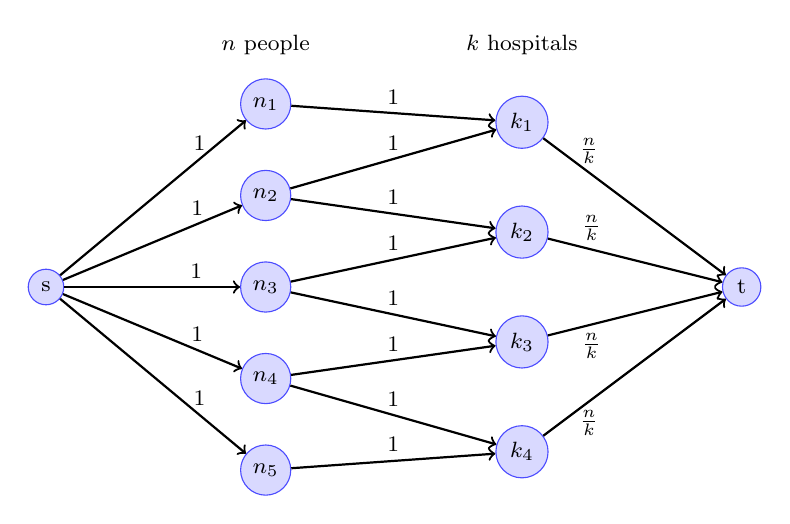
\begin{tikzpicture}[scale=0.93, node/.style = {circle, draw=blue!70, fill=blue!15,
	minimum size=4mm, inner sep=1.0mm}, edge/.style = {thick, ->}]

	\node (source) [node] at (-5cm, 0cm) {s};

	\node (n1) [node] at (-2cm, 2.50cm) {$n_1$};
	\node (n2) [node] at (-2cm, 1.25cm) {$n_2$};
	\node (n3) [node] at (-2cm, 0.00cm) {$n_3$};
	\node (n4) [node] at (-2cm,-1.25cm) {$n_4$};
	\node (n5) [node] at (-2cm,-2.50cm) {$n_5$};

	\draw[edge] (source) -- node [above, near end] {1} (n1);
	\draw[edge] (source) -- node [above, near end] {1} (n2);
	\draw[edge] (source) -- node [above, near end] {1} (n3);
	\draw[edge] (source) -- node [above, near end] {1} (n4);
	\draw[edge] (source) -- node [above, near end] {1} (n5);

	\node (k1) [node] at (1.5cm, 2.25cm) {$k_1$};
	\node (k2) [node] at (1.5cm, 0.75cm) {$k_2$};
	\node (k3) [node] at (1.5cm,-0.75cm) {$k_3$};
	\node (k4) [node] at (1.5cm,-2.25cm) {$k_4$};

	\draw[edge] (n1) -- node [above] {1} (k1);
	\draw[edge] (n2) -- node [above] {1} (k1);
	\draw[edge] (n2) -- node [above] {1} (k2);
	\draw[edge] (n3) -- node [above] {1} (k2);
	\draw[edge] (n3) -- node [above] {1} (k3);
	\draw[edge] (n4) -- node [above] {1} (k3);
	\draw[edge] (n4) -- node [above] {1} (k4);
	\draw[edge] (n5) -- node [above] {1} (k4);

	\node (sink) [node] at (4.5cm, 0cm) {t};

	\draw[edge] (k1) -- node [above, near start] {$\frac{n}{k}$} (sink);
	\draw[edge] (k2) -- node [above, near start] {$\frac{n}{k}$} (sink);
	\draw[edge] (k3) -- node [below, near start] {$\frac{n}{k}$} (sink);
	\draw[edge] (k4) -- node [below, near start] {$\frac{n}{k}$} (sink);

	% Descriptions
	\node at (-2.0cm, 3.3cm) {$n$ people};
	\node at ( 1.5cm, 3.3cm) {$k$ hospitals};
\end{tikzpicture}

\begin{itemize}
	\item The flow along an edge can not exceed its capacity
	\item The net flow from $u$ to $v$ must be the opposite of the net flow
		from $v$ to $u$. (What goes in, must come out)
	\item The flow leaving the source $s$ must be equal to the flow
		arriving at the sink $t$.
\end{itemize}

The min cut is equal to the max flow in a flow network.

\textbf{Ford--Fulkerson}:
$\mathcal{O}(\vert{E}\vert f)$, $f$ is the maximum flow. \\
\textbf{Edmonds--Karp}: (a variation of Ford--Fulkerson):
$\mathcal{O}(\vert{V}\vert \vert{E}\vert^2)$.



\section{NP}
$$ Y \leq_p X $$
$Y$ is polynomial-time reducible to $X$, or $X$ is at least as hard as
$Y$ (with respect to polynomial time).

\begin{definition}
	Suppose $Y \leq_p X$. If $X$ can be solved in polynomial time, then $Y$
	can be solved in polynomial time.
\end{definition}

\subsection{NP-Complete problems}
To prove that a problem $Y$ is NP-complete you have to:
\begin{enumerate}
	\item Show that you can verify a solution to $Y$ in polynomial time.
		($Y \in$ NP)
	\item Give a reduction $A$ from some NP-complete problem $X$ to $Y$.
	\item Prove that $s \in X \Leftrightarrow A(s) \in Y$.
\end{enumerate}
\columnbreak
\subsubsection{List of problems}
\begin{tabular}{l l}
Packing                 & Independent Set \\
                        & Set Packing \\
Covering                & Vertex Cover \\
                        & Set Cover \\
Partitioning            & 3-Dimensional Matching \\
                        & Graph Coloring \\
Sequencing              & Hamiltonian Path/Cycle \\
                        & Traveling Salesman \\
Numerical               & Subset Sum \\
Constraint Satisfaction & 3-Sat \\
\end{tabular}


\section{Graphs}
$G(V, E)$

\subsection{Breadth-First-Search}
Perhaps the simplest algorithm for determining $s-t$ connectivity is
breadth-first search (BFS), in which we explore outward from $s$ in all
possible directions, adding nodes one ''layer'' at a time. Thus we start with
$s$ and include all nodes that are joined by an edge to $s$ -- this is the first
layer of the search. We then include all additional nodes that are joined
by an edge to any node in the first layer -- this is the second layer. We
continue in this way until no new nodes are encountered. 
Time complexity: $\mathcal{O}(\vert{V}\vert + \vert{E}\vert)$.

\subsection{Depth-First-Search}
Another natural method to find the nodes reachable from $s$ is the approach
you might take if the graph $G$ were truly a maze of interconnected rooms
and you were walking around in it. You'd start from $s$ and try the first
edge leading out of it, to a node $v$. You'd then follow the first edge
leading out of $v$, and continue in this way until you reached a ''dead
end'' -- a node for which you had already explored all its neighbors. You'd
then backtrack until you got to a node with an unexplored neighbor, and
resume from there. We call this algorithm depth-first search (DFS), since
it explores $G$ by going as deeply as possible and only retreating when
necessary. Time complexity: $\mathcal{O}(\vert{V}\vert + \vert{E}\vert)$.

\section{Minimum Spanning Tree}
A subset of the edges that forms a tree that includes every vertex,
where the total weight of all the edges in the tree is minimized.

\subsection{Prim's algorithm}
\begin{enumerate}
	\item Initialize a tree with a single vertex, chosen arbitrarily from the graph.
	\item Grow the tree by one edge: of the edges that connect the tree to
		vertices not yet in the tree, find the minimum-weight edge, and
		transfer it to the tree.
	\item Repeat step 2 (until all vertices are in the tree).
\end{enumerate}
Time complexity when using binary heap priority queues and adjacency list:
$\mathcal{O}(\vert{E}\vert \log \vert{V}\vert)$.


\vfill
\rule{0.38\linewidth}{0.4pt} \\
You made this? I made this -- \author

\end{multicols*}
\end{document}
